\documentclass[aspectratio=169]{beamer}

\usetheme{Madrid}
\usecolortheme{default}
\setbeamertemplate{navigation symbols}{}
\setbeamertemplate{footline}[frame number]
\setbeamercolor{structure}{fg=blue!60!black}
\setbeamercolor{frametitle}{fg=black,bg=blue!8}
\setbeamersize{text margin left=0.8cm, text margin right=0.8cm}

\usepackage[T1]{fontenc}
\usepackage[utf8]{inputenc}
\usepackage{lmodern}
\usepackage{amsmath}
\usepackage{amssymb}
\usepackage{mathtools}
\usepackage{graphicx}
\usepackage{tikz}
\usetikzlibrary{arrows.meta}
\usepackage{xcolor}

\title{Inverse Functions and One-to-One Functions}
\author{Section Media Workflow}
\date{}

\begin{document}

\begin{frame}[t]{Why Study Inverse Functions?}
\textbf{Goal.} See why reversing a process leads naturally to one-to-one functions.

\begin{itemize}
  \item A function can be viewed as a process that sends an input \(x\) to an output \(y=f(x)\).
  \item Some formulas should be reversible, such as converting Celsius to Fahrenheit and back again.
  \item A reversible rule needs each output to come from exactly one input.
\end{itemize}
\end{frame}

\begin{frame}[t]{Definition of a One-to-One Function}
\textbf{Goal.} Recognize the formal condition that makes a function invertible.

\begin{itemize}
  \item Different inputs must produce different outputs.
  \item The equivalent implication form is often the easier test in practice.
  \item This is the key property that allows a function to have an inverse.
\end{itemize}

\[
f(x_1)\ne f(x_2)
\qquad \text{whenever } x_1\ne x_2.
\]

\[
f(x_1)=f(x_2) \implies x_1=x_2.
\]
\end{frame}

\begin{frame}[t]{A Real-World One-to-One Test}
\textbf{Goal.} Apply the definition to ordinary processes before moving to algebraic functions.

\begin{itemize}
  \item Student ID numbers are unique, so the function is one-to-one.
  \item Blood types repeat across students, so that function is not one-to-one.
  \item The test is always the same: can one output belong to more than one input?
\end{itemize}

\[
f(\text{student})=\text{Student ID number}
\]

\[
g(\text{student})=\text{Blood type}.
\]
\end{frame}

\begin{frame}[t]{Why \(x^2\) Can Fail To Be Invertible}
\textbf{Goal.} See exactly how repeated outputs prevent an inverse from being well defined.

\begin{itemize}
  \item \(f(x)=x\) on \([0,1]\) is one-to-one, but \(g(x)=x^2\) on \([-1,1]\) is not.
  \item The output \(\frac14\) comes from both \(\frac12\) and \(-\frac12\).
  \item \(g^{-1}\!\left(\frac14\right)\) is not well defined on the full interval \([-1,1]\).
\end{itemize}

\[
f(x)=x, \qquad 0\le x\le 1,
\]

\[
g(x)=x^2, \qquad -1\le x\le 1.
\]

\[
g\left(\frac12\right)=\left(\frac12\right)^2=\frac14
\qquad \text{and} \qquad
g\left(-\frac12\right)=\left(-\frac12\right)^2=\frac14.
\]
\end{frame}

\begin{frame}[t]{The Horizontal Line Test}
\textbf{Goal.} Connect the definition of one-to-one with a geometric test on the graph.

\begin{itemize}
  \item A horizontal line represents a fixed output value \(y=c\).
  \item If the graph is hit twice, then two inputs share the same output.
  \item So a function is one-to-one exactly when every horizontal line meets the graph at most once.
\end{itemize}

\[
f(x_1)=c=f(x_2).
\]
\end{frame}

\begin{frame}[t]{Horizontal Line Test: Visual Check}
\textbf{Goal.} Read the horizontal line test directly from a graph.

\centering
\begin{minipage}{0.46\textwidth}
\centering
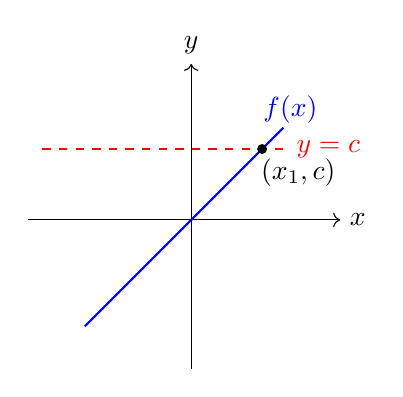
\begin{tikzpicture}[scale=0.9]
\draw[->] (-2.3,0) -- (2.1,0) node[right] {$x$};
\draw[->] (0,-2.1) -- (0,2.2) node[above] {$y$};
\draw[blue, thick] (-1.5,-1.5) -- (1.3,1.3);
\draw[red, dashed] (-2.1,1) -- (1.3,1);
\fill (1,1) circle (2pt);
\node[blue] at (1.4,1.55) {$f(x)$};
\node[below right] at (0.85,1) {$(x_1,c)$};
\node[red, right] at (1.35,1) {$y=c$};
\end{tikzpicture}

\vspace{0.4em}
One-to-one function\\
Intersects at most once.
\end{minipage}
\hfill
\begin{minipage}{0.46\textwidth}
\centering
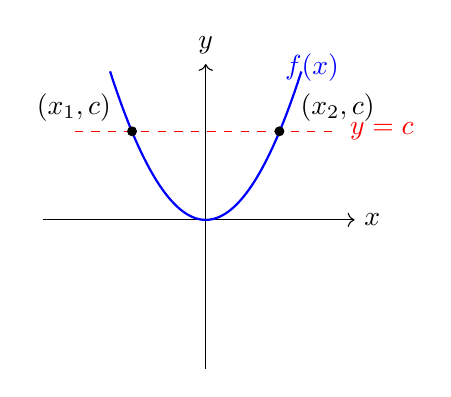
\begin{tikzpicture}[scale=0.9]
\draw[->] (-2.3,0) -- (2.1,0) node[right] {$x$};
\draw[->] (0,-2.1) -- (0,2.2) node[above] {$y$};
\draw[blue, thick, domain=-1.35:1.35, samples=100] plot (\x,{1.15*\x*\x});
\draw[red, dashed] (-1.85,1.25) -- (1.85,1.25);
\fill (-1.04,1.25) circle (2pt);
\fill (1.04,1.25) circle (2pt);
\node[blue] at (1.5,2.15) {$f(x)$};
\node[above left] at (-1.2,1.25) {$(x_1,c)$};
\node[above right] at (1.2,1.25) {$(x_2,c)$};
\node[red, right] at (1.9,1.25) {$y=c$};
\end{tikzpicture}

\vspace{0.4em}
Not one-to-one\\
Intersects more than once.
\end{minipage}
\end{frame}

\begin{frame}[t]{Definition of an Inverse Function}
\textbf{Goal.} Describe an inverse as a function that reverses the original correspondence.

\begin{itemize}
  \item If \(f\) sends \(x\) to \(y\), then \(f^{-1}\) sends \(y\) back to \(x\).
  \item The domain and range switch roles when we pass to the inverse.
  \item Using \(x\) as the input variable for \(f^{-1}\) is only a notation change, not a new idea.
\end{itemize}

\[
f^{-1}(y)=x
\quad \Longleftrightarrow \quad
f(x)=y,
\qquad y\in B.
\]

\[
f^{-1}(x)=y
\quad \Longleftrightarrow \quad
f(y)=x.
\]
\end{frame}

\begin{frame}[t]{When Does an Inverse Exist?}
\textbf{Goal.} Use the theorem that completely characterizes when an inverse exists.

\begin{itemize}
  \item A function has an inverse function if and only if it is one-to-one.
  \item Being one-to-one is both necessary and sufficient.
  \item Quick checks: \(f(x)=x\) and \(g(x)=x^3\) are both invertible.
\end{itemize}

\[
    f^{-1}(x)=x.
    \]

\[
    g^{-1}(x)=\sqrt[3]{x}.
    \]
\end{frame}

\begin{frame}[t]{Three Steps For Finding An Inverse}
\textbf{Goal.} Use the standard algebraic procedure for computing inverse functions.

\begin{itemize}
  \item Write \(y=f(x)\).
  \item Solve this equation for \(x\) in terms of \(y\).
  \item Interchange \(x\) and \(y\) to obtain \(f^{-1}(x)\).
\end{itemize}
\end{frame}

\begin{frame}[t]{Example: Finding The Inverse Of \(x^3+2\)}
\textbf{Goal.} Apply the three-step procedure to a function that is already one-to-one.

\begin{itemize}
  \item Start with \(y=x^3+2\) and solve for \(x\).
  \item After isolating \(x\), interchange the variables.
  \item A composition check confirms the answer.
\end{itemize}

\[
y=x^3+2.
\]

\[
x=\sqrt[3]{\,y-2\,}.
\]

\[
f^{-1}(x)=\sqrt[3]{\,x-2\,}.
\]
\end{frame}

\begin{frame}[t]{Example: Restricting The Domain Of \(x^2\)}
\textbf{Goal.} See how a domain restriction can create an inverse for a function that was not invertible before.

\begin{itemize}
  \item On \([0,\infty)\), the function \(f(x)=x^2\) becomes one-to-one.
  \item We choose the nonnegative square root because the original domain requires \(x\ge 0\).
  \item Restricting the domain can make an inverse possible.
\end{itemize}

\[
y=x^2,
\qquad x\ge 0.
\]

\[
x=\sqrt{y}.
\]

\[
f^{-1}(x)=\sqrt{x},
\qquad x\ge 0.
\]
\end{frame}

\begin{frame}[t]{Checking An Inverse By Composition}
\textbf{Goal.} Use the composition identities to verify that a candidate inverse really works.

\begin{itemize}
  \item \(f^{-1}(f(x))=x\) for every \(x\in A\).
  \item \(f(f^{-1}(x))=x\) for every \(x\in B\).
  \item These identities are the standard verification step after solving for an inverse.
\end{itemize}

\begin{center}
\resizebox{\textwidth}{!}{%
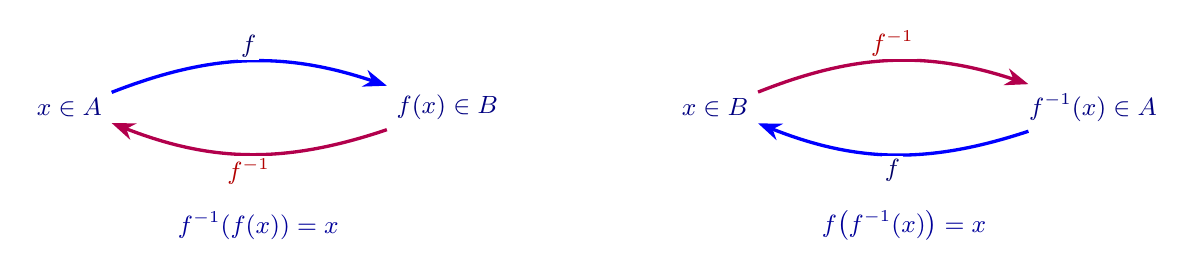
\begin{tikzpicture}[
        transform shape,
        >=Stealth,
        every node/.style={font=\small},
        lab/.style={midway, fill=white, inner sep=1pt},
        mainnode/.style={text=blue!50!black},
        fwd/.style={->, very thick, draw=blue!50!blue},
        bwd/.style={->, very thick, draw=red!70!blue}
    ]

    \node[mainnode] (xA) at (0,0) {$x\in A$};
    \node[mainnode] (fxB) at (4.8,0) {$f(x)\in B$};

    \draw[fwd, bend left=20] (xA) to node[lab, above, text=blue!40!black] {$f$} (fxB);
    \draw[bwd, bend left=20] (fxB) to node[lab, below, text=red!70!black] {$f^{-1}$} (xA);

    \node[text=blue!60!black] at (2.4,-1.5) {$f^{-1}(f(x))=x$};

    \node[mainnode] (xB) at (8.2,0) {$x\in B$};
    \node[mainnode] (finvxA) at (13,0) {$f^{-1}(x)\in A$};

    \draw[bwd, bend left=20] (xB) to node[lab, above, text=red!70!black] {$f^{-1}$} (finvxA);
    \draw[fwd, bend left=20] (finvxA) to node[lab, below, text=blue!40!black] {$f$} (xB);

    \node[text=blue!60!black] at (10.6,-1.5) {$f\bigl(f^{-1}(x)\bigr)=x$};

    \end{tikzpicture}
}
\end{center}
\end{frame}

\end{document}
